\paragraph{3.1} \textbf{Non-computable processes in Nature}%%%%%%%%%%%%%%%%%%%%%%%%%%%%%%%%%%%%%%%%%%%%
\\

Since we know that a Turing Machine only maps from non-negative to non-negative numbers, and if any process in nature is found to map between different sets of values then that process can't be run on a Turing Machine.


\paragraph{3.2} \textbf{Turing numbers }
\\
Taking the input of the Turing Machine $a_1,...,a_k$ and then give the Turing machine the value $p_1^{a_1} \times p_2^{a_2} \times ..... \times p_k^{a_k}$ withe $p_1, p_2, p_3,...p_k$ being the first $k$ prime numbers, and thus all Turing machine with unique inputs will be given unique value identifiers since all numbers only have one kind of prime factorization.

\paragraph{3.3} \textbf{Turing Machine to reverse a bit string}
\\
Our aim is to design a Turing Machine to reverse a binary string consisting of $0$ and $1$, we will call them $a$ and $b$

\begin{itemize}
    \item Move the last digit , replace $x$ for $a$ or $x$ for $b$ and move right to convert the corresponding $B$ to $a$ or $b$ accordingly.

    \item Move left until the symbol left to $x$ is reached.

    \item Perform Step 1 and Step 2 until $B$ is reached while traversing left.

    \item Replace every $x$ to $B$ to make the cells empty since the reverse string is performed by the previous steps.
\end{itemize}

The transition diagram for the Turing machine looks like this

\begin{figure}
    \centering
    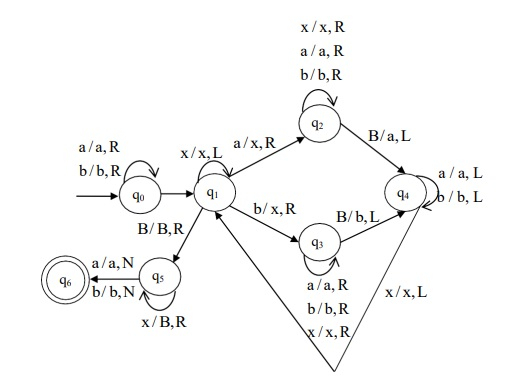
\includegraphics[ width = \linewidth]{Chapter 3/reverse_string.jpg}
    \caption{The Turing Machine for reverse string}
    \label{fig:my_label}
\end{figure}

\paragraph{3.4} \textbf{Turing Machine to add modulo 2}
\\
\begin{itemize}
    

\item  Start in the initial state, with the tape head positioned over the leftmost digit of the first number.
\item  If the digit under the tape head is 0, move the tape head one position to the right and transition to the next state.
\item  If the digit under the tape head is 1, write a 0 at that position and move the tape head one position to the right.
\item Repeat steps 2 and 3 until the tape head reaches the rightmost digit of the first number.
\item  Transition to the next state and move the tape head to the leftmost digit of the second number.
\item  Repeat steps 2-4 for the second number.
\item  Move the tape head to the leftmost digit of the result and transition to the final state.

\end{itemize}

This Turing machine will add two binary numbers modulo 2, effectively performing a bitwise XOR operation on the input numbers.



\paragraph{3.5} \textbf{Halting Problem with no inputs}

\\

The problem of determining whether a given Turing machine halts when the input to the machine is a blank tape is known as the halting problem. It was shown by Alan Turing in 1936 that there is no general algorithm that can determine whether an arbitrary Turing machine halts on a blank input.

The proof of this result relies on the concept of diagonalization, where a new machine is constructed that can determine whether any given machine halts on a blank input. If such an algorithm existed, then it could be encoded as a Turing machine, say H. It is possible to construct a new machine, say D, that takes as input the description of another machine M and runs both M and H on the blank tape. D compares the outputs of M and H for each machine it receives as input. If the outputs are different for any input machine M, D outputs "M does not halt." Otherwise, D outputs "M halts."

The problem is that D can be used to determine whether itself halts. If D halts, it will say "D halts." If D does not halt, it will say "D does not halt." This creates a contradiction, because D cannot simultaneously halt and not halt. Therefore, it is impossible for a machine to determine whether another machine halts on a blank input.

This proof was shown by Alan Turing in his paper "On computable numbers, with an application to the Entscheidungsproblem" in 1936, showing that the halting problem is undecidable.
\\

Define H2(M) = {0  if the machine doesn't halt with blank input 
, 1  if the machine does halt with a blank input}

We have the following algorithm

$\textit{Turing(M)}$\\
$\textit{Y = H2(M)}$ \\
$\textit{if } y== 0$ \\ 
    $ \textit{halt}$\\
$\textit{else}$\\
`$\textit{Loop Forever}$\\

Here if $M$ is blank, then $H2(M) = 1$ only if $y = H2(M) = 0$ , thus we form a contradiction, meaning this machine cannot read input $M$, which is blank, meaning there is no algorithm to solve $H2(M)$ for this particular machine.


\paragraph{3.6} \textbf{Probabilistic halting problem}
\\

Define Hp(x) = {$0$ if probability machine $x$ halts in input $x<1/2$, $1$ if probability $ > 1/2$ }
We have the following algorithm:

Turing(x) \\
Y = hp(x) \\
Y2 = flip an unbiased coin \\
if y==1 and y2 = heads \\
halt \\
Else \\
loop forever \\
End if\\

Here, assume hp(x) = 1 and thus corresponding probability $p > 1/2$. The probability program halts are $p \times 1/2 =$ at most $1/2$ since $p$ is at most $1$. Thus, this contradicts our original statement that hp(x) = 1, and thus there is no algorithm to correctly determine hp(x) for this machine.

\paragraph{3.7} \textbf{Halting oracle}
\\

Yes. Before, the problem was no algorithm existed to compute HALT(x) for all x, but now that the black box exists that algorithm also exists, and since Turing machines can compute all algorithms, these Turing machines can compute this algorithm for all machines.

\paragraph{3.8} \textbf{Universality of NAND}
\\

AND - input bit $[1,x_0, x_1]$. Apply NAND to $x_0$ and $x_1$ , then a NAND on $[1, \text{NAND}(x_0, x_1)$] \\
NOT - NAND input bit $x_0$ and ancilla bit $1$ \\
XOR - input $[1,x_0, x_1,1,1]$ NAND$[1,\text{NAND}[x_0,x_1]$,  NAND[NAND[$1, x_0$] NAND[$1, x_1$]]]


\paragraph{3.9} \textbf{Prove that $f(n)$ is $O(g(n))$ iff $g(n)$ is $\Omega(f(n))$}
\\

$f(n)$ is $O(g(n)) \rightarrow f(n) \le cg(n)$ \\
$g(n)$ is $\Omega(f(n)) \rightarrow cf(n) \le g(n)$ \\
If $g(n)$ is $\Omega(f(n))$ then $cf(n) \le g(n), f(n) \le g(n) /c$ \\
And thus $f(n) \le cg(n)$ and $f(n)$ is $O(g(n))$ \\

Thus $g(n)$ is $\Theta(f(n))$ and $f(n)$ is $O(g(n))$

\paragraph{3.10} \textbf{Suppose $g(n)$ is a polynomial of degree $k$}
\\

$$ g(n) \text{is} O(n^1) \longrightarrow g(n) \le cn^1$$
$$g(n) = An^k + Bn^{k-1} + .... + d \le cn^1$$
Thus, because $An^k + Bn^{k-1}+...+ d \le n^{k+1} \le n^{k+2}$ and we design $c$ such that $An^k + Bn^{k-1}+...+ d \le cn^k$, thus $g(n)$ is $O(n^1)$.

\paragraph{3.11} \textbf{Show that $\log$(n) is $O(n^k)$ for any $k >0$}
\\

$\log n \le cn^k$, $n \le c 10^{n^k}$, so we design $c^k$ such that $n \le c\times 10^{n^k}$ for all $k>0$

\paragraph{3.12} \textbf{$n^{\log n}$ is super polynomial}
\\

From 3.10 , we proved $\log n \ge k$ for sufficiently large $n$, thus $g(n) = n^k$ is in $O(n^{\log  n})$. However, $\log n$ is not $ \le k$ for large $n$, so $g(n) = n^k$ is never in $O(n^k)$


\paragraph{3.13} \textbf{$n^{\log n}$ is sub-exponential}
\\

$c^n$  is $\Omega(n^{\log n})$, check graphically for sufficiently large $n$.

Since $c^n$ is $\Omega(n^{\log n})$ , $n^{\log n}$ can't be in $\Omega(c^n)$.

\paragraph{3.14} \textbf{Suppose $e(n)$ is $O(f(n))$ and $g(n)$ is $O(h(n))$}
\\

$$e(n) \text{ is } O(f(n)) \rightarrow e(n) \le cf(n)$$
$$ g(n) \text{ is } O(h(n)) \rightarrow g(n) \le c2\times h(n)$$ 
$$ e(n) \times g(n) \le c\times c2 \times f(n) \times h(n) = c3 \times f(n) \times h(n)$$

\paragraph{3.15} \textbf{Lower bound for compare and swap based sorts}
\\

After $1$ swapping, there is only $2^1$ ordering such that the swapping puts the whole thing in order. After $2$ swapping, there are $2^2$ orderings that were two swapping away from being sorted. After $k$ swappings, it follows that $2^k$ initial orderings are now sorted. 
        
$$ 2^n \log n = 2^{\log n^n = n^{n}} \ge n! $$
        
Thus, the lower bound on sorting is $ n \log n$. You can see that asymptotic notations have the important effect of allowing us to find how efficient a particular algorithm can be on a process, but it doesn’t necessarily tell us HOW to make such an algorithm, but it gives us an idea of how efficient the most efficient algorithm can be. 





\paragraph{3.16} \textbf{Hard to compute function exist}
\\
There exist Boolean functions on $n$ inputs which require at least $2^n/\log(n)$ logic gates to compute. One such example is the function known as the "n-input majority function."

The majority function, denoted as $MAJ_n(x_1, x_2, ..., x_n)$, is a Boolean function that takes $n$ binary inputs and outputs $1$ if and only if more than $n/2$ of the inputs are $1$. The function can be computed by creating n AND gates, one for each input, and $n-1$ OR gates to combine the outputs of the AND gates. In the worst case, where all inputs are $1$, the number of gates required is $(n-1) + (n-1) = 2n - 2 = 2^n/log(n)$ gates.

Another example is the "n-input parity function," which is a Boolean function that takes n binary inputs and outputs $1$ if and only if the number of 1s in the inputs is odd. The function can be computed by creating n XOR gates, one for each input, and then $n-1$ XOR gates to combine the outputs of the previous XOR gates. In the worst-case scenario, the number of gates required is $(n-1) + (n-1) = 2n - 2 = 2^n/log(n)$ gates.

This shows that there are Boolean functions that require at least $2^n/log(n)$ logic gates to compute, and that is a lower bound for the complexity of some Boolean functions.

\paragraph{3.17} \textbf{Prove that a polynomial-time algorithm for finding the factors of a number $m$ exists iff the factoring decision problem is in P}
\\

If this problem is in $P$, then a Turing machine exists for identifying if a value is a factor of a number m and less than $L$, and thus setting $L = m$ we have the factoring algorithm that can thus be done efficiently. If this problem isn’t in $P$, the factoring obviously can’t be done efficiently since if for any $L$ it is inefficient then $L=m$ is definitely inefficient. 


\paragraph{3.18} \textbf{Prove that if $coNP \ne NP$, then $P \ne NP$}
\\

$P$ is a subset of $CoNP$ so if $CoNP$ does not equal $NP$, there are some problems in $P$ and $CoNP$, and the rest of the problems in $P$ and $NP$, and thus there are some problems in $P$ that are in $CoNP$ but not $NP$ and thus $P$ does not equal $NP$.

\paragraph{3.19} \textbf{The REACHABILITY problem}
\\

Start at the first vertex, try to get to the 2nd. At most $n$ vertices exist to visit, so its $O(n)$(algorithm would make sure not to visit a vertice more than once). 
        Then use Reachability algorithm to form the following $O(n^2)$ algorithm:
                \\ For $i$ through all vertices
                        \\ For $j$ through all vertices
                                \\ Test Reachability(vertex(i), vertex(j)
                        \\ End $j$
                \\ End $i$


\paragraph{3.20} \textbf{Euler's Theorem}
\\

Euler’s theorem is based on the following idea: If you visit a node, you can go on a new edge you haven’t gone before, because the vertex has an even amount of incident edges so if a node is visited and then left, 2 edges have been traversed and used. Thus if you go through all nodes you will always have a new edge to move through for every node until there are no more edges left to visit, at which point you are back at the original node and have completed the cycle. 

The procedure then would be to start at a node, go to all other nodes until you have reached back to the original node and there are no new edges to visit.

\paragraph{3.21}\textbf{Transitive property of reduction}
\\
Since $L1 -> L2$ exists, there exists function $R(x)$ that gives a string in language $L2$ iff $x$ is in $L1$. Since $L2 -> L3$ exists, there exists a function $R2(x_2)$ that gives a string in $L3$ iff $x_2$ is in $L2$. Thus, with $R(x) + R2(R(x))$ (polynomial time overhead), we reduce $L1$ to $L3$.

\paragraph{3.22} \textbf{$L$ is complete}
\\
Since all other problems can be reduced to L, and L can be reduced to L’, all other problems can be reduced to L’. 




\paragraph{3.23} \textbf{SAT is NP-complete problem}
\\

SAT (Satisfiability) is a problem of determining whether a given Boolean formula, in conjunctive normal form (CNF) has a satisfying assignment.

First, to show that SAT is in NP, we need to show that a solution to the problem can be verified in polynomial time. Given a Boolean formula in CNF and an assignment, we can check in polynomial time if the assignment satisfies the formula, by checking each clause of the formula. If all the clauses are true for the given assignment, then the assignment is a satisfying assignment, otherwise not. Since the size of the input does not affect the time complexity of the verification, this means that SAT is in NP.

Next, to show that SAT is NP-complete, we need to show that there exists a reduction from an arbitrary problem in NP to SAT. One such problem is known as CSAT (Circuit SAT), which is the problem of determining whether a given Boolean circuit has a satisfying assignment.

To show that CSAT reduces to SAT, we can construct a Boolean formula in CNF that represents the given Boolean circuit. Each gate in the circuit can be represented by a clause in the CNF formula, and each input to the circuit can be represented by a variable in the formula. We can then use the variables to represent the inputs and the clauses to represent the gates, such that the Boolean formula in CNF is satisfied if and only if the circuit has a satisfying assignment.

Since CSAT is in NP and it is possible to reduce it to SAT, it implies that SAT is NP-complete. This means that SAT is at least as hard as any problem in NP, and that any problem in NP can be reduced to SAT in polynomial time.

\paragraph{3.25} \textbf{PSPACE subset EXP}
\\

With $lm^{p(n)}$ different states, all problems in PSPACE can be solved by going through all possible states in $lm^{p(n)}$ time, or exponential time. Thus PSPACE is a subset of EXP

\paragraph{3.26} \textbf{L subset P}
\\

If you can solve a problem in $L$, then you can solve the problem by going through around $c \times log(n)$ spaces, thus you can solve it in time $c \times log(n)$, which is polynomial. Thus $L$ is a subset of $P$.

\paragraph{3.27} \textbf{Approximation algorithm for VERTEX COVER}
\\

In this algorithm, at worst the min vector span is made up of all the alpha’s and none of the Beta’s, in which case at worst this algorithm calculates the a vector span that is $2 \times$ the space of the min vector span.

\paragraph{3.29} \textbf{Fredkin gate is self inverse}
\\

A Fredkin gate is a reversible gate that acts on three qubits, and it is also known as a Controlled-SWAP gate. The Fredkin gate is defined as:

$$|x⟩|y⟩|z⟩ → |x⟩|y⟩|z⟩ if \text{x} = 0$$
$$|x⟩|y⟩|z⟩ → |x⟩|z⟩|y⟩ \text{if} x = 1$$

Where $|x⟩$, $|y⟩$ and $|z⟩$ are the input qubits and |x⟩, |y⟩, |z⟩ are the output qubits. The qubit x is the control qubit, and the qubits y and z are the target qubits.

Now, let's consider applying two consecutive Fredkin gates, where the first one acts on qubits |x⟩, |y⟩, |z⟩ and the second one acts on qubits |x⟩, |z⟩, |w⟩.

If x = 0, the first Fredkin gate doesn't change the state of the qubits and the second Fredkin gate also don't change the state of the qubits, and the output state is |x⟩|y⟩|z⟩|w⟩ which is the same as the input state |x⟩|y⟩|z⟩|w⟩

If x = 1, the first Fredkin gate swaps the qubits |y⟩ and |z⟩, and the second Fredkin gate swaps the qubits |z⟩ and |w⟩. The net effect is that the qubits |y⟩ and |w⟩ are swapped and the output state is |x⟩|w⟩|z⟩|y⟩ which is the same as the input state |x⟩|y⟩|z⟩|w⟩

Therefore, applying two consecutive Fredkin gates gives the same outputs as inputs


\paragraph{3.32} \textbf{From fredkin to toffoli}
\\
e a Fredkin gate?
The Toffoli gate, also known as the Controlled-Controlled-NOT gate, is a reversible gate that acts on three qubits. The Toffoli gate is defined as:

$$|x⟩|y⟩|z⟩ → |x⟩|y⟩|z⟩ \text{ if } x = 0 \text{ and } y = 0 $$
$$|x⟩|y⟩|z⟩ → |x⟩|y⟩|z \otimes 1⟩ \text{ if } x = 0 \text{ and } y = 1$$

where |x⟩, |y⟩, and |z⟩ are the input qubits and |x⟩, |y⟩, |z⟩ are the output qubits. The qubits x and y are the control qubits, and the qubit z is the target qubit.

The smallest number of Fredkin gates needed to simulate a Toffoli gate is 3. To simulate a Toffoli gate with three Fredkin gates, we can use a technique called 'controlled-SWAP-controlled-SWAP', where the first two Fredkin gates act on |x⟩, |y⟩, |z⟩ and the third Fredkin gate acts on |x⟩, |y⟩, |t⟩ where |t⟩ is an auxiliary qubit.

On the other hand, Toffoli gate is a more powerful gate than Fredkin gate and it can simulate Fredkin gate, but it requires 2 Toffoli gates to simulate 1 Fredkin gate. To simulate a Fredkin gate with two Toffoli gates, we can use a technique called "controlled-controlled-NOT-controlled-NOT" where the first Toffoli gate is applied on |x⟩, |y⟩, |t1⟩ where |t1⟩ is an auxiliary qubit, and the second Toffoli gate is applied on |x⟩, |t1⟩, |z⟩

It's important to note that while it's possible to simulate a Toffoli gate using Fredkin gates, or vice versa, it's not always the most efficient way to perform the operation, as the number of gates required for the simulation is higher than using the native gate.